\newpage
\ifthenelse {\boolean{bachelor}}
{
	%\section{Results}
	\section{Experimenty}
}
{
	%\chapter{Results}
	\chapter{Experimenty}
}
\label{experiments}
Na systéme boli vykonané tri experimenty. V prvom experimente bol systém porovnaný so systémom na sumarizáciu textu. Druhý experiment overoval použitie pravidiel na základe štruktúry viet. Posledný bol používateľský experiment, počas ktorého bol náš systém testovaný reálnymi používateľmi.

\subsection{Porovnanie systému}
\label{experiments:first_experiment}
V prvom experimente sme náš systém použili na spracovanie troch článkov z wikipádie~\footnote{www.simple.wikipedia.org}. Výsledky sme porovnali s Autosummarizer~\footnote{www.autosummarizer.com}, systémom zameraným na sumarizáciu textu, využívajúci extrakčnú sumarizáciu. Články obsahovali spolu 27 viet a 294 slov.

\subsubsection{Výsledky}
\label{experiments:first_experiment:results}
Porovnali sme počty viet a slov na výstupe systémov. Počty sú na~\imgref{experiments:first_experiment:results:fig:output}. V časti \textit{a} je zobrazený počet viet a v časti \textit{b} je počet slov. V druhej časti porovnania sme sa zamerali na prístup systémov k spracovaniu viet a slov. Na~\imgref{experiments:first_experiment:results:fig:processing} v časti \textit{a} je zobrazený počet viet, ktoré systémy nespracovali a v časti \textit{b} je priemerný počet eliminovaných irelevantných slov vo výslednej vete. 

\begin{figure}[H]%
	\centering
	\subfloat[Počet viet na výstupe]{{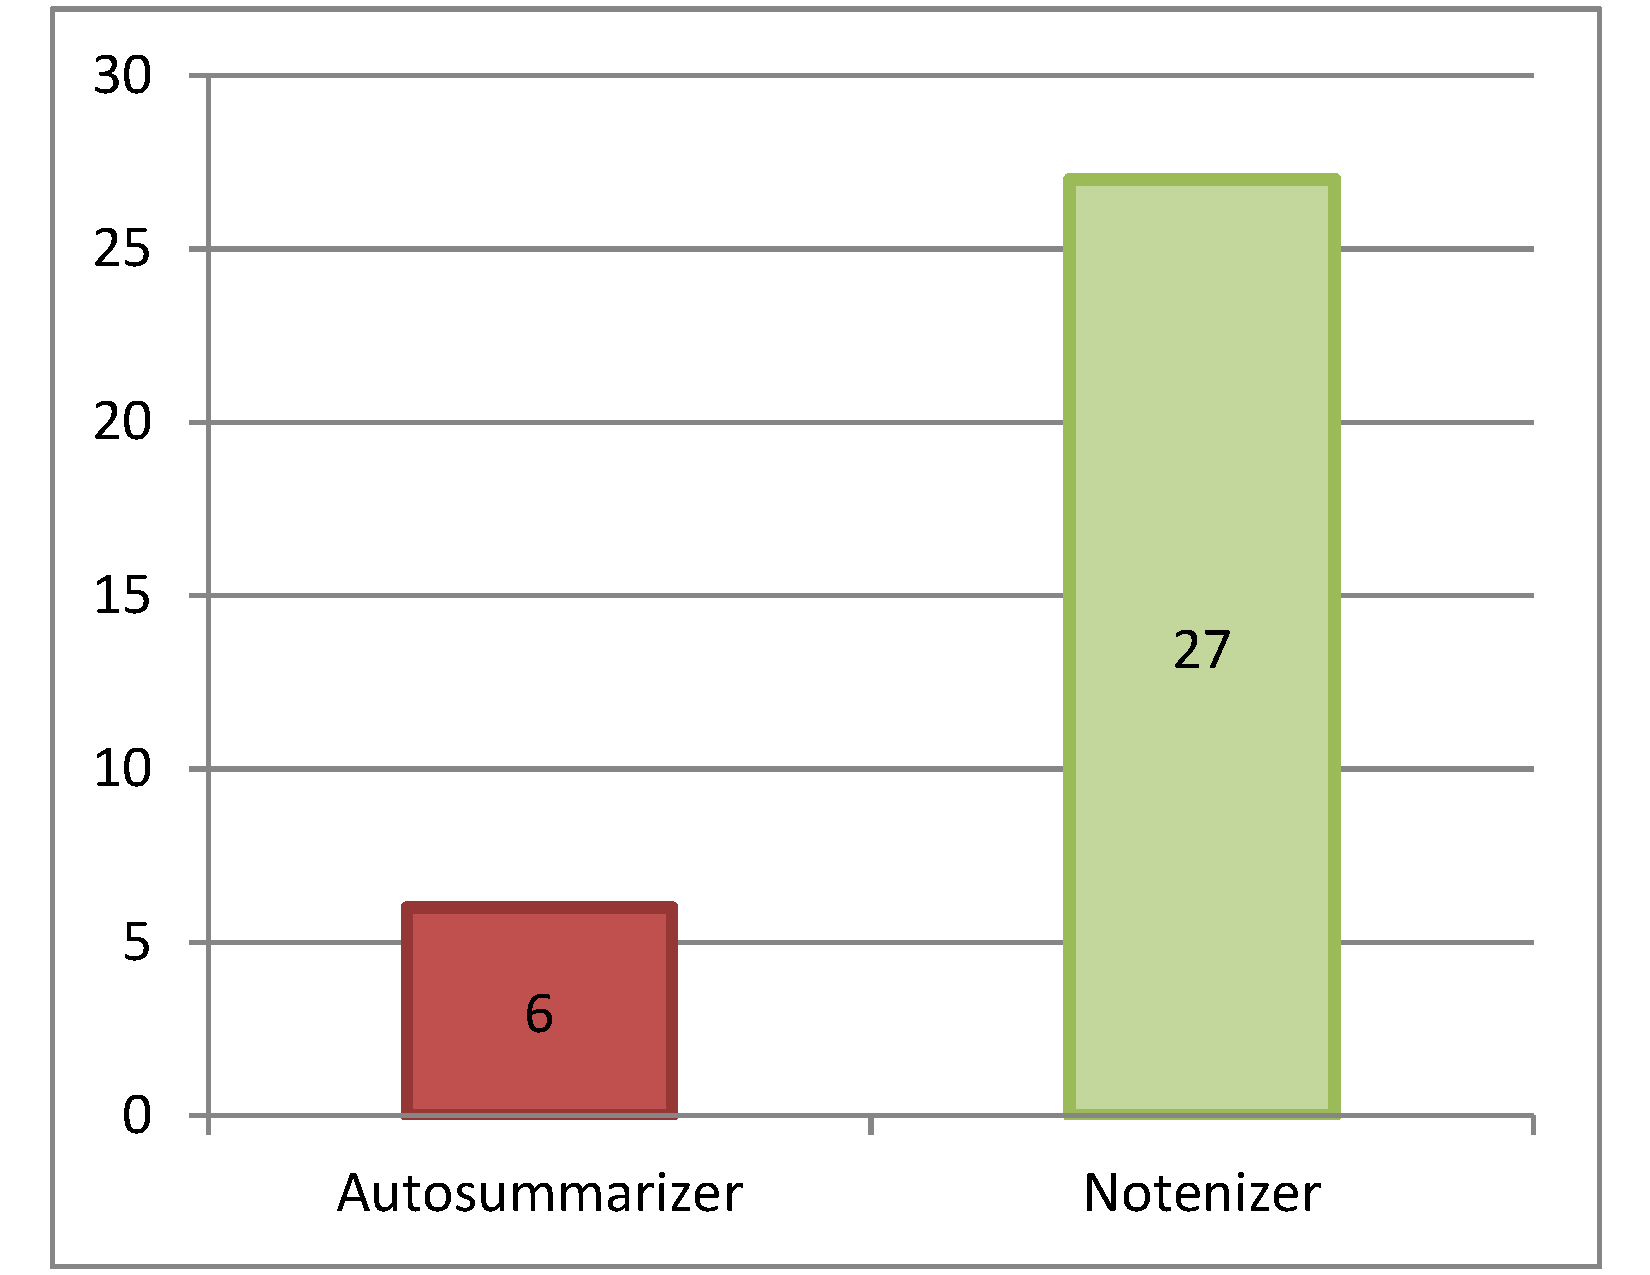
\includegraphics[scale=0.22]{exp_exp_sentences_output} }}%
	\qquad
	\subfloat[Počet slov na výstupe]{{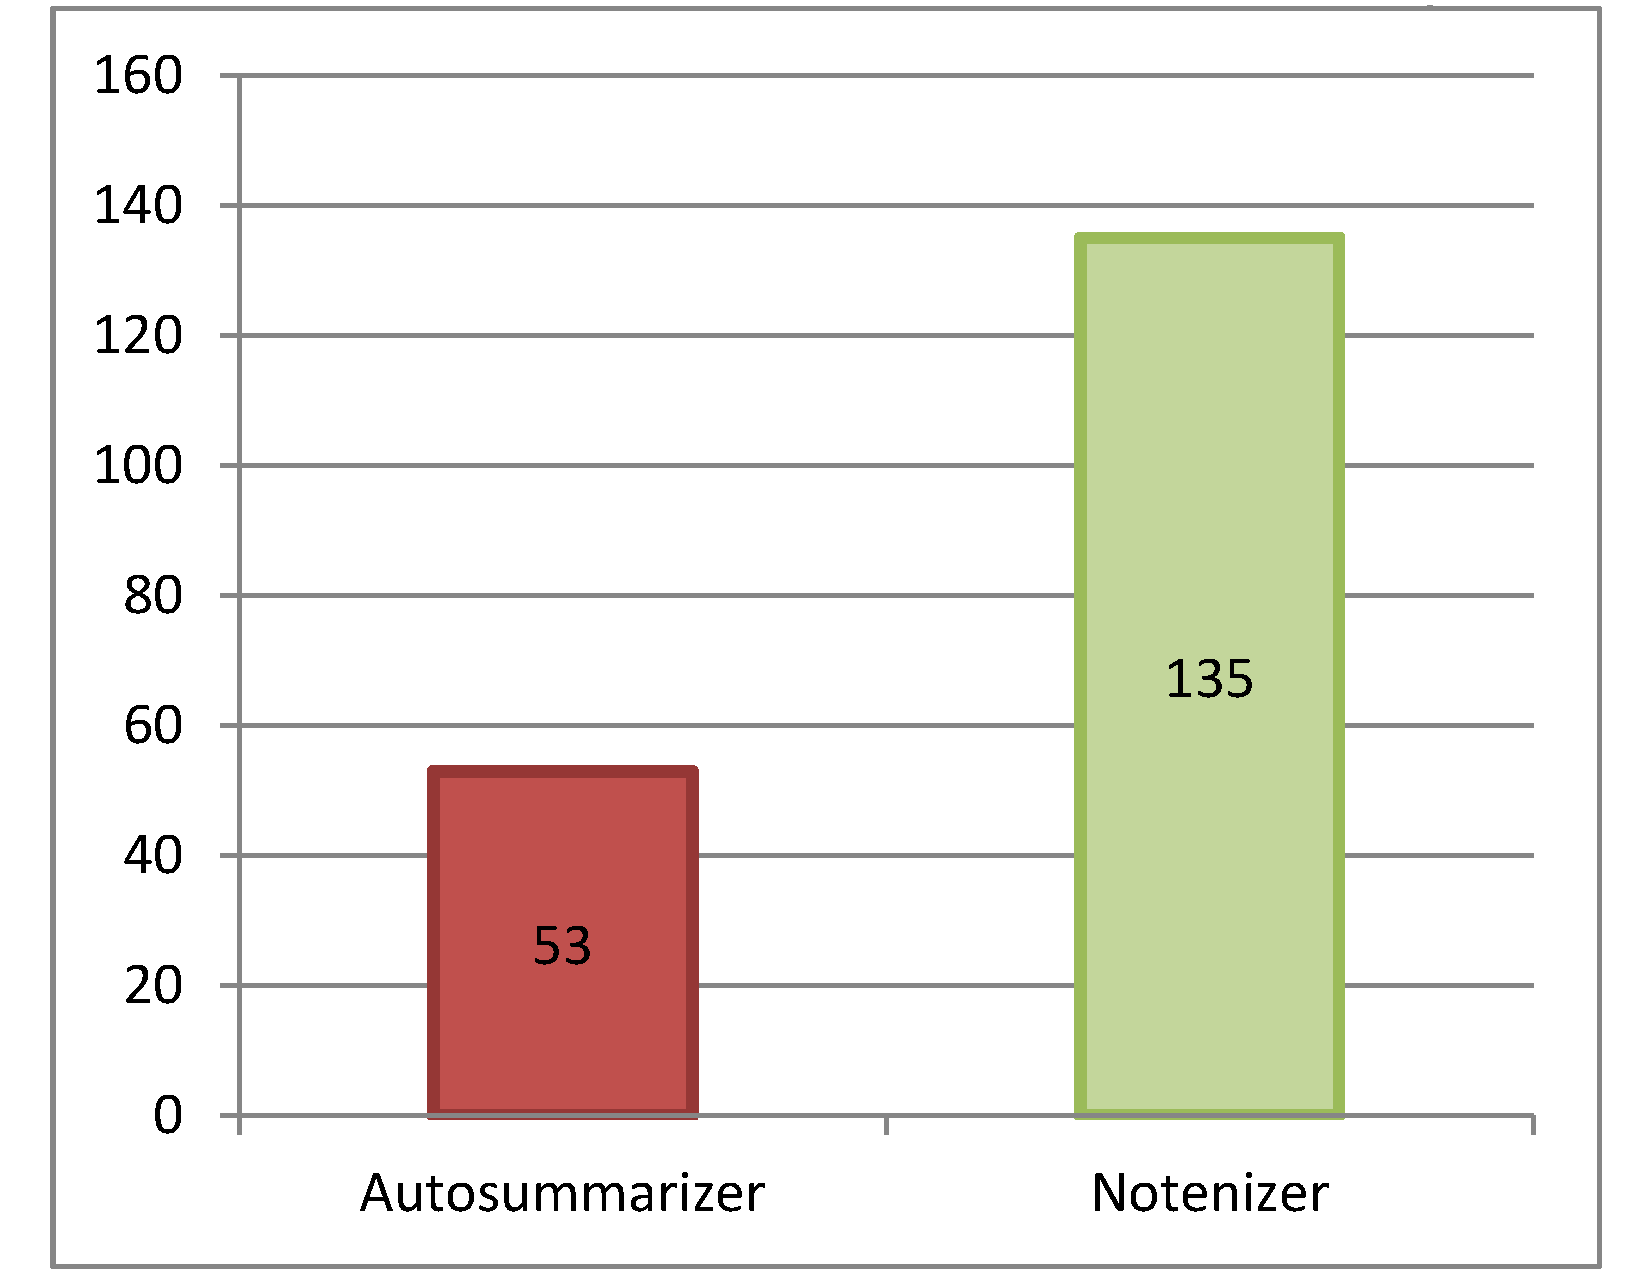
\includegraphics[scale=0.22]{exp_exp_words_output} }}%
	\caption{Výstupy porovnaných systémov}%
	\label{experiments:first_experiment:results:fig:output}%
\end{figure}

\begin{figure}[H]%
	\centering
	\subfloat[Počet nespracovaných viet]{{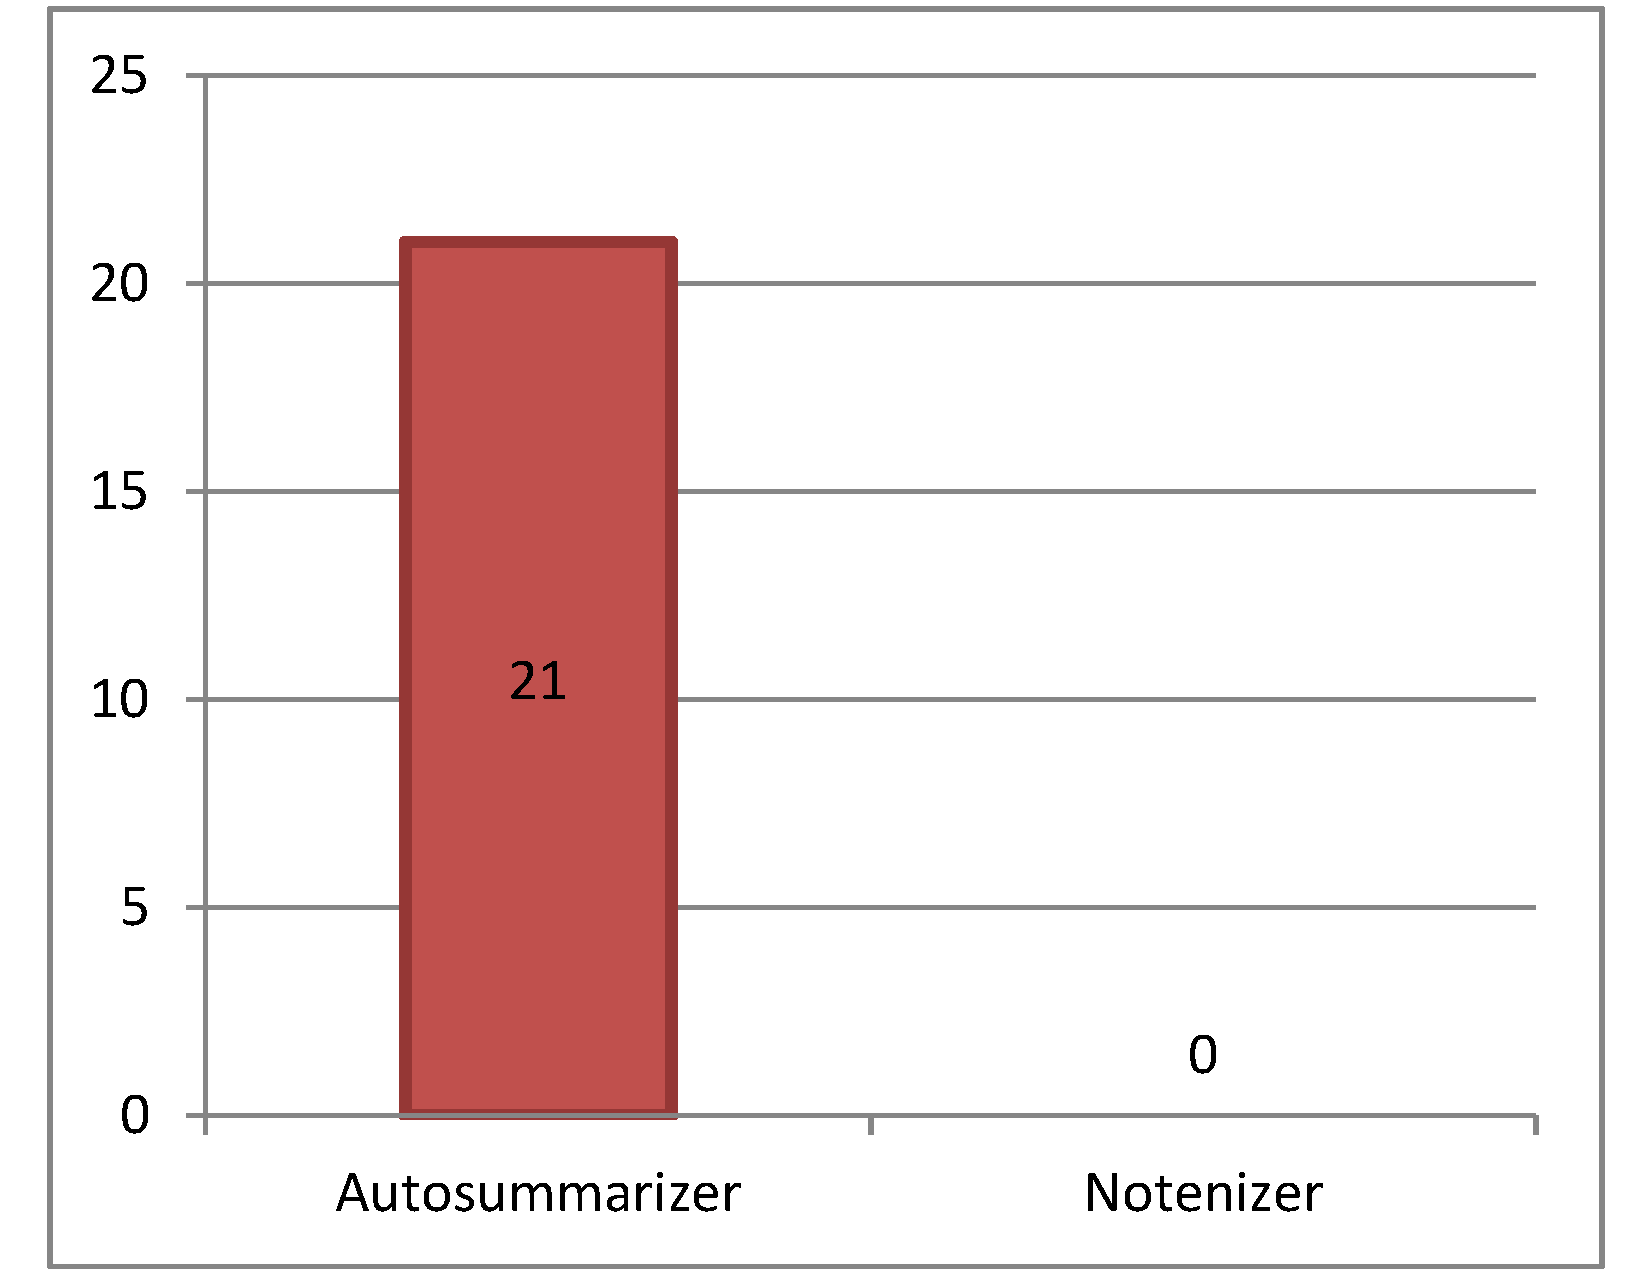
\includegraphics[scale=0.22]{exp_exp_sentences_not_processed} }}%
	\qquad
	\subfloat[Priemerný počet eliminovaných irelevantných slov vo výslednej vete]{{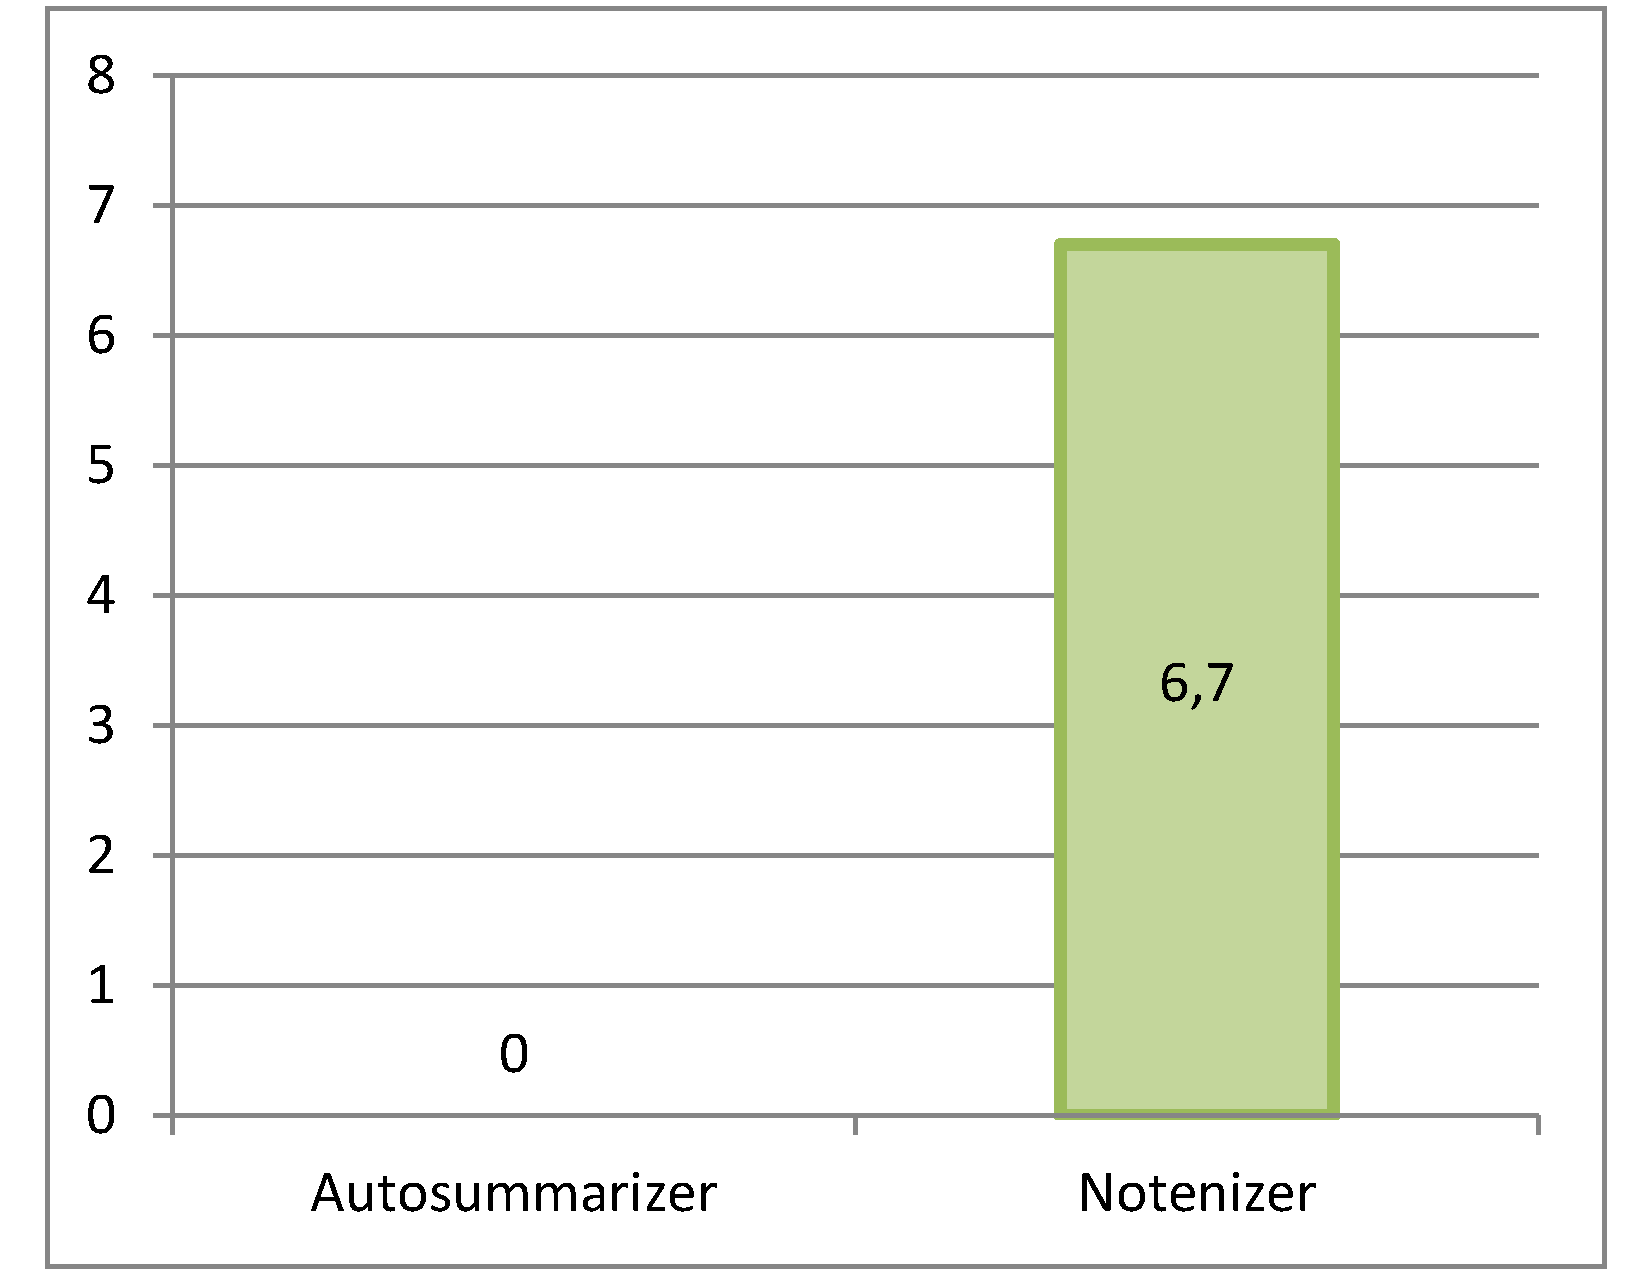
\includegraphics[scale=0.22]{exp_exp_irrelevant_words_eliminated_avg} }}%
	\caption{Spracovanie informácií porovnanými systémami}%
	\label{experiments:first_experiment:results:fig:processing}%
\end{figure}

\subsubsection{Vyhodnotenie porovnania}
Autosummarizer systém dosahoval lepšie výsledky v menšom počte viet a slov na výstupe, ale kvôli tomu vynechal veľa relevantných informácií. Náš systém na výstupe zobrazoval väčšie množstvo slov a viet, avšak spracoval všetky vety a eliminoval z nich irelevantné informácie, slová.

\subsection{Použitie pravidiel}
Otestovali sme aplikovateľnosť pravidiel závislých od štruktúry vety. Pri spracovaní $340$ viet z tridsiatich článkov bolo potrebné vytvoriť a použiť $263$ pravidiel. Z toho vyplýva, že pri $77$ vetách bolo aplikované pravidlo na základe štruktúry vety a nebolo potrebné vytvárať nové. To predstavuje približne $22,65\%$ všetkých viet, čím sa nám podarilo práve takéto množstvo pravidiel ušetriť.

\subsection{Používateľský experiment}
\label{experiments:main_experiment}
Na používateľskom experiment sa zúčastnilo pätnásť študentov, ktorí v systéme spracovali článok a získali z neho poznámky. Množina článkov experimentu pozostávala z článkov z wikipédie\footnote{www.simple.wikipedia.org} o štátoch z Európy. Účastník experimentu si zvolil článok, ktorý sa následne spracoval. Experiment sa skladal z dvoch častí. V prvej časti sa článok vybraný účastníkom spracoval nad databázou, ktorá obsahovala počet pravidiel z piatich vopred spracovaných článkov. V druhej časti sa ten istý článok spracoval nad databázou s tridsiatimi vopred spracovanými článkami. Účastník v oboch častiach experimentu vytvorené poznámky z viet článku ohodnotil, prípadne upravil. Všetci účastníci testovali systém nad databázami s rovnakými dátami. Počas experimentu bolo spracovaných pätnásť článkov s $236$ vetami.

\subsubsection{Výsledky}
\label{experiments:main_experiment:results}
Na~\imgref{experiments:user_experiment:results:fig:exp_general_comparison} sú zobrazené pomery správnych a nesprávnych vytvorených poznámok. Na časti \textit{a} tohoto obrázka vidno pomer pri spracovaní článku v prvej časti experimentu a v časti \textit{b} je pomer z druhej časti experimentu.

\begin{figure}[H]%
	\centering
	\subfloat[Všeobecné výsledky prvej časti]{{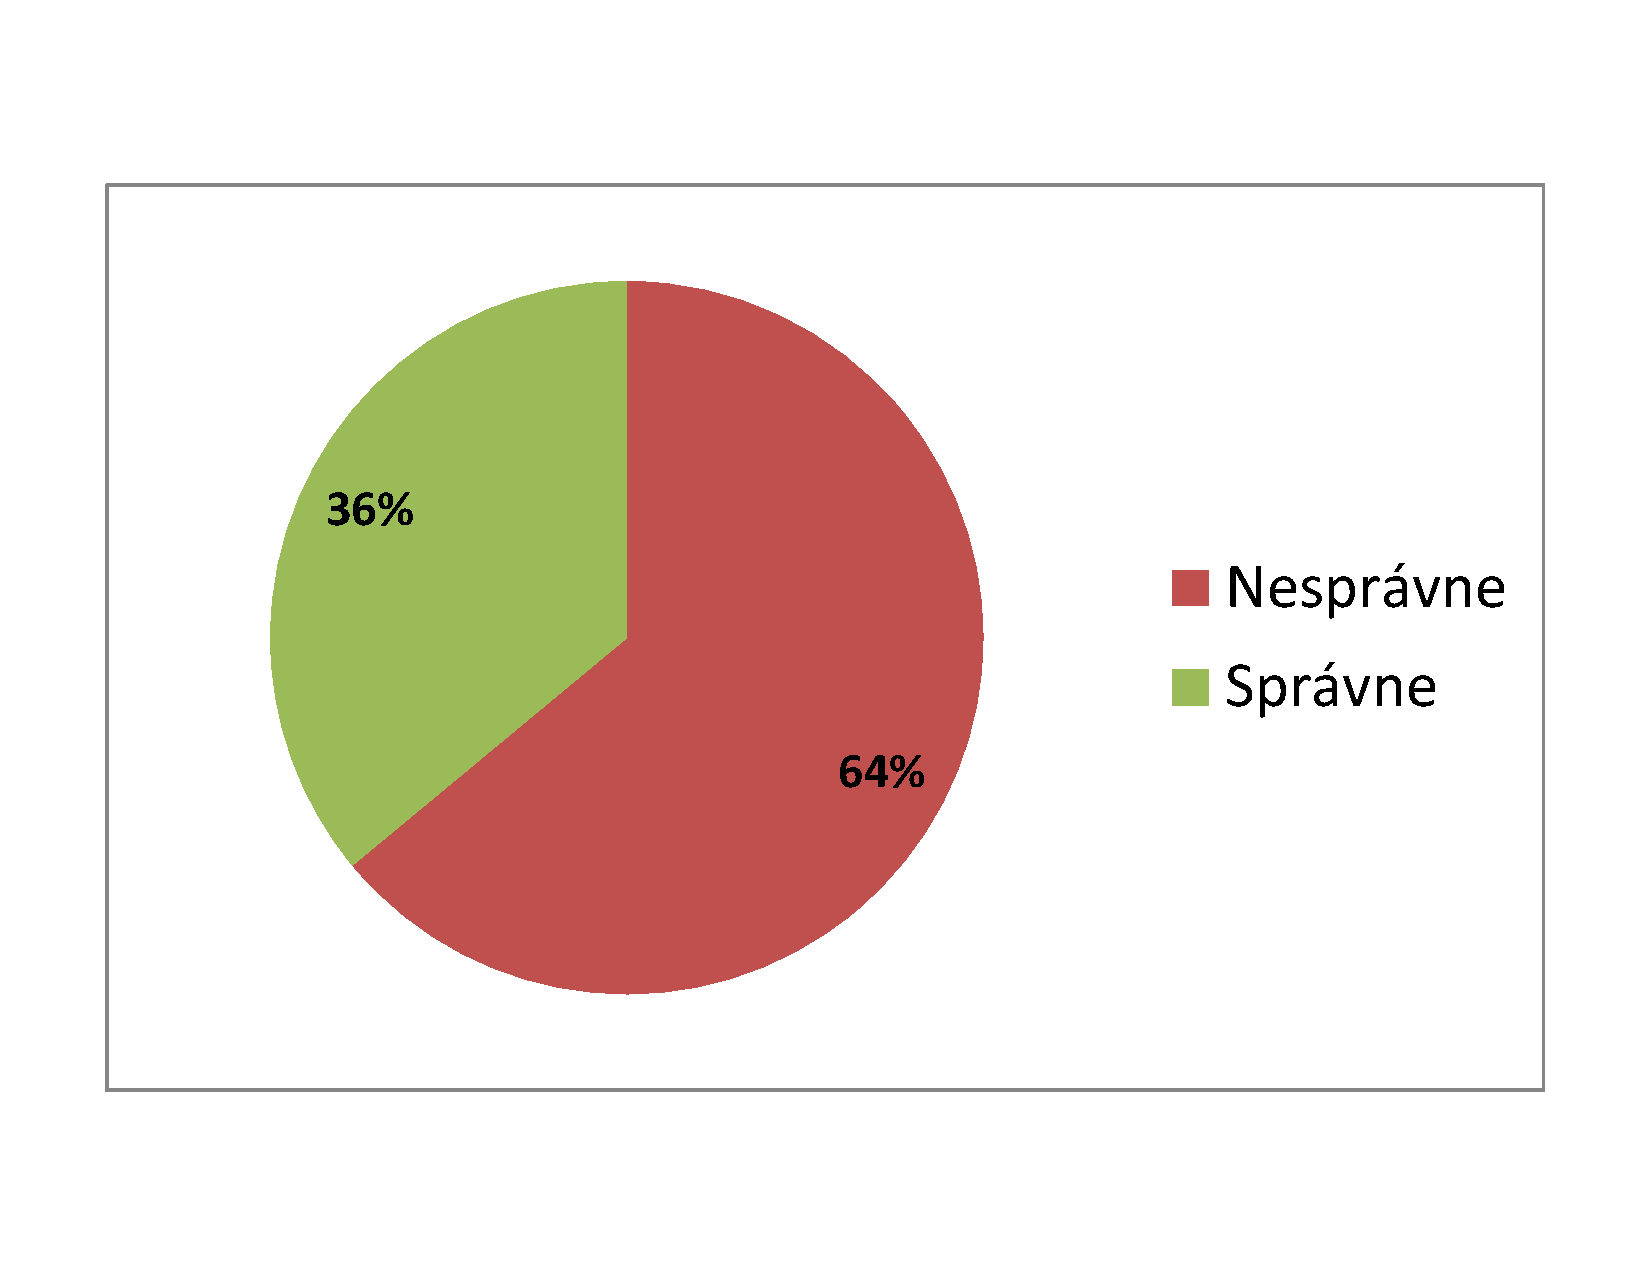
\includegraphics[scale=0.29]{exp_first_general} }}%
	\qquad
	\subfloat[Všeobecné výsledky druhej časti]{{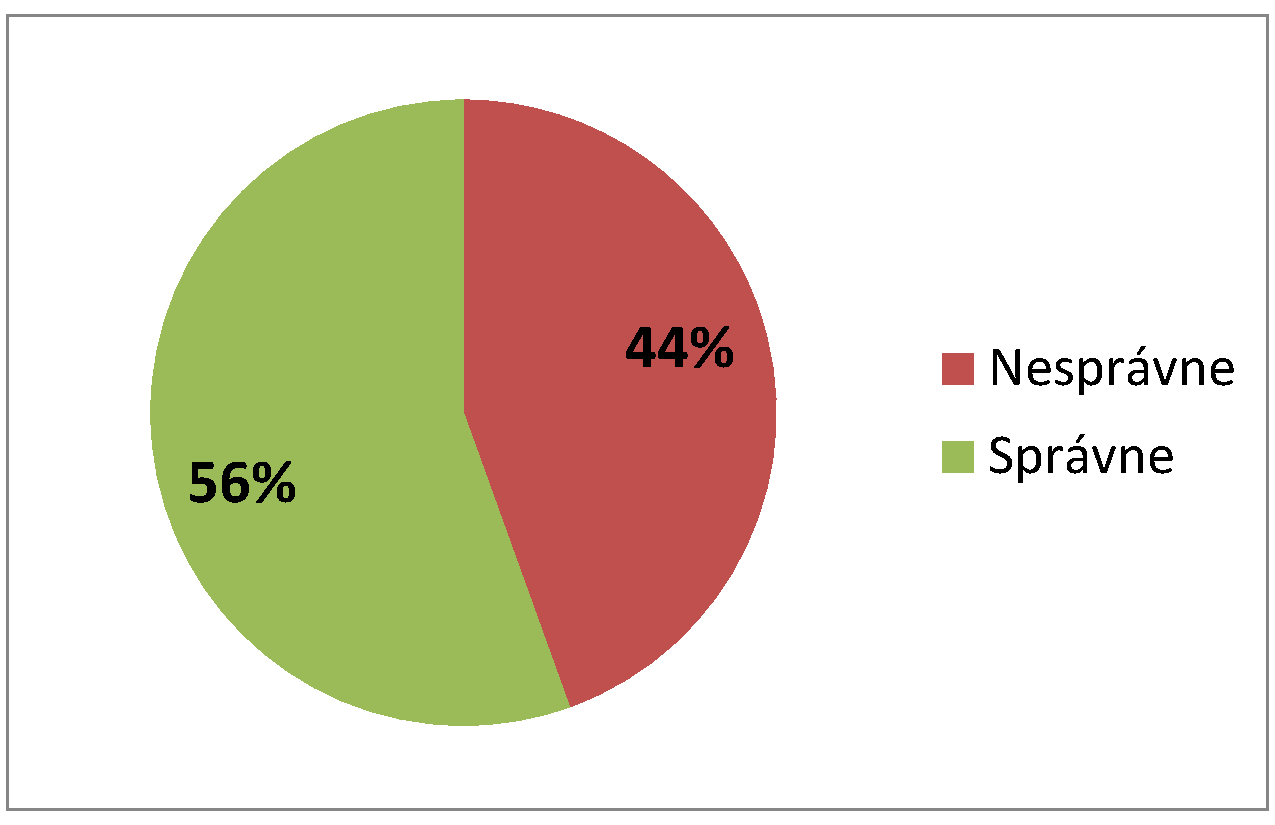
\includegraphics[scale=0.29]{exp_second_general} }}%
	\caption{Porovnanie všeobecných výsledkov oboch časti experimentu}%
	\label{experiments:user_experiment:results:fig:exp_general_comparison}%
\end{figure}

Správne aj nesprávne poznámky boli podľa hodnotení účastníkov kategorizované do štrnástich kategórií. Najpočetnejšie z nich sú pre nesprávne poznámky \textit{zlé spracované, chýba podstatná informácia, chýba mala časť informácie} a pre správne poznámky sú to \textit{správne, OK - zlý slovosled, OK - subjektívne}.

\textit{Zle spracované} znamená, že systém zle spracoval vetu a vytvorená poznámka neobsahovala takmer žiadnu informáciu a nedávala zmysel. V kategórií \textit{chýba podstatná informácia} sú zaradené poznámky, ktoré boli korektne vytvorené, avšak chýbala v nich podstatná informácia z vety potrebná na jej pochopenie. V poznámkach, ktoré obsahovali veľkú časť podstatnej informácie, prípadne celú podstatnú informáciu, ale chýbala v nej malá časť informácie z pôvodnej vety potrebná na to, aby sa dala považovať za správnu poznámku, boli zaradené do kategórie \textit{chýba mala časť informácie}. Do kategórie \textit{správne} boli zaradené poznámky, ktoré boli správne vytvorené. Kategória \textit{OK - zlý slovosled} obsahuje poznámky, ktoré obsahovali celú podstatnú informáciu z vety, ale slovosled vety bol zlý. Poznámky, ktoré boli označené za správne, ale účastník sa vyjadril, že si vie predstaviť, že pre niekoho by daná poznámka nemusela byť správna, boli zaradené do kategórie \textit{OK - subjektívne}.

Na~\imgref{experiments:user_experiment:results:fig:exp_detailed_comparison_first} a~\imgref{experiments:user_experiment:results:fig:exp_detailed_comparison_second} sú zobrazené percentuálne zastúpenia kategórií pri prvej a druhej časti experimentu, v tomto poradí.

\begin{figure}[H]%
	\centering
	\subfloat[Kategórie nesprávnych poznámok]{{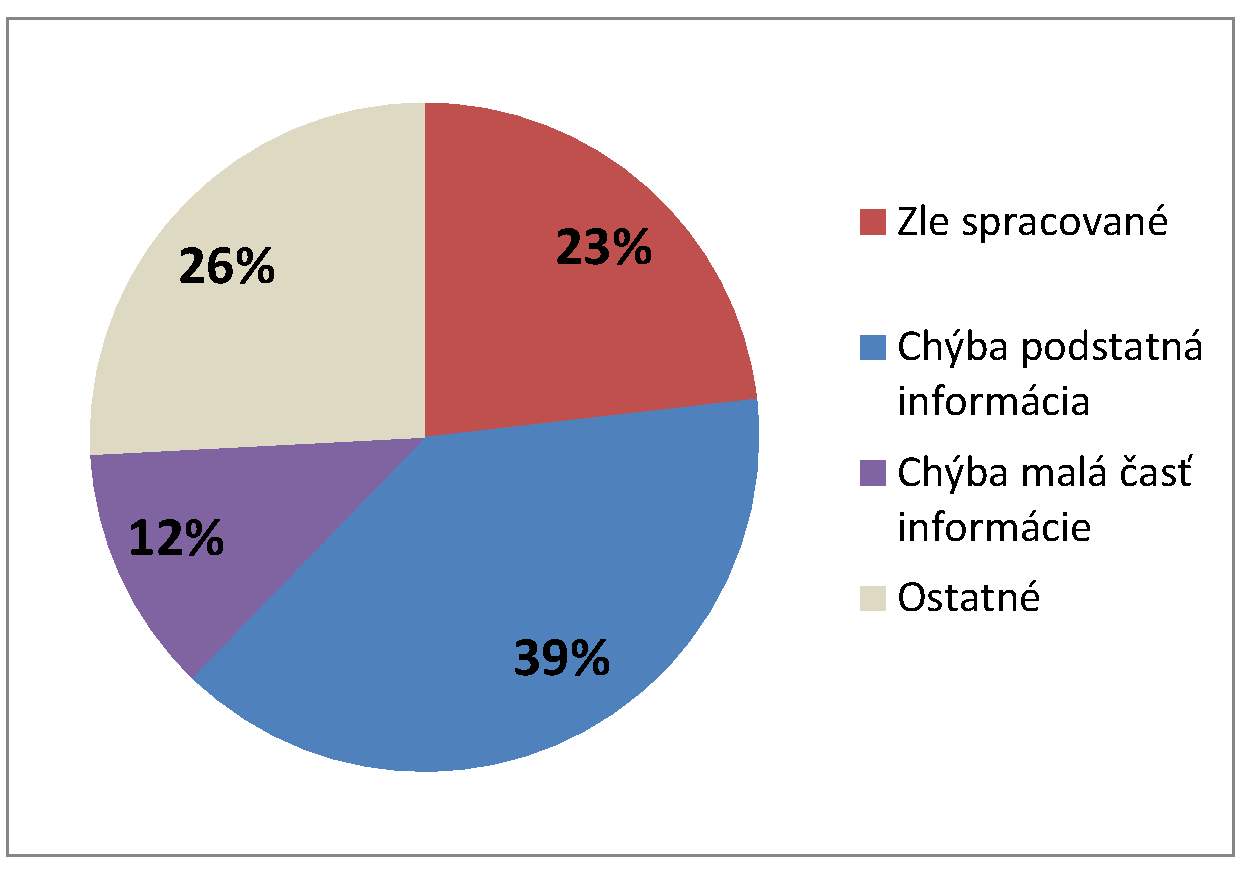
\includegraphics[scale=0.30]{exp_first_wrong} }}%
	\qquad
	\subfloat[Kategórie správnych poznámok]{{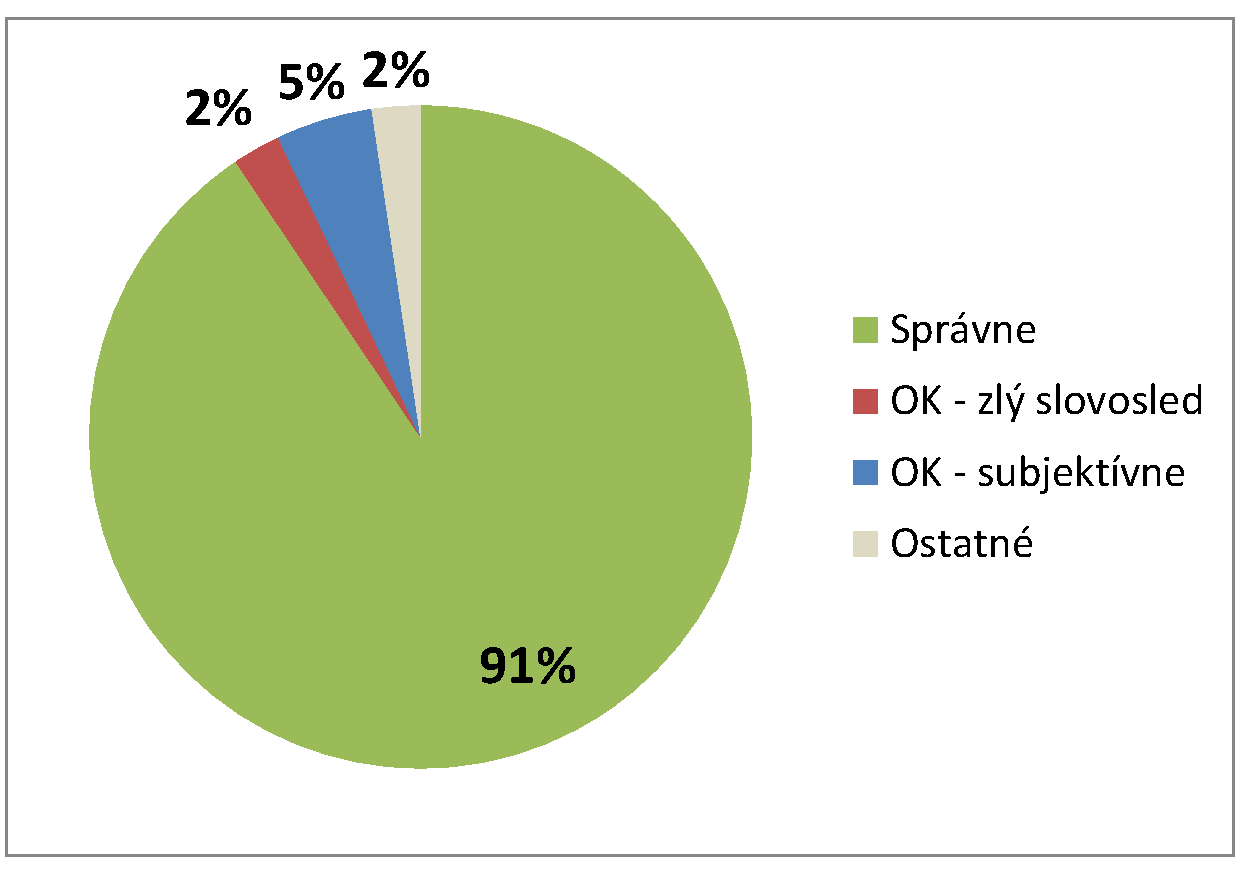
\includegraphics[scale=0.30]{exp_first_correct} }}%
	\caption{Detailné výsledky prvej časti experimentu}%
	\label{experiments:user_experiment:results:fig:exp_detailed_comparison_first}%
\end{figure}


\begin{figure}[H]%
	\centering
	\subfloat[Kategórie nesprávnych poznámok]{{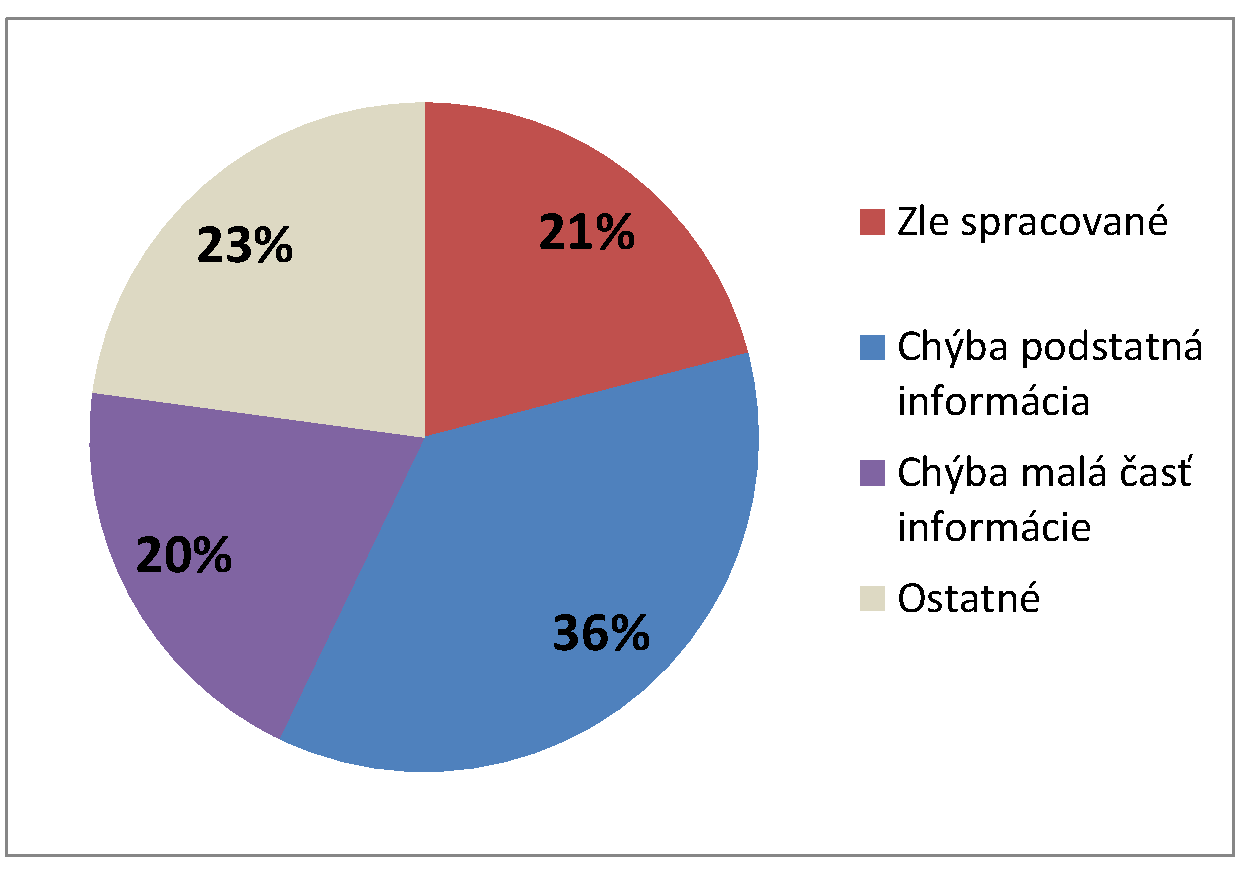
\includegraphics[scale=0.30]{exp_second_wrong} }}%
	\qquad
	\subfloat[Kategórie správnych poznámok]{{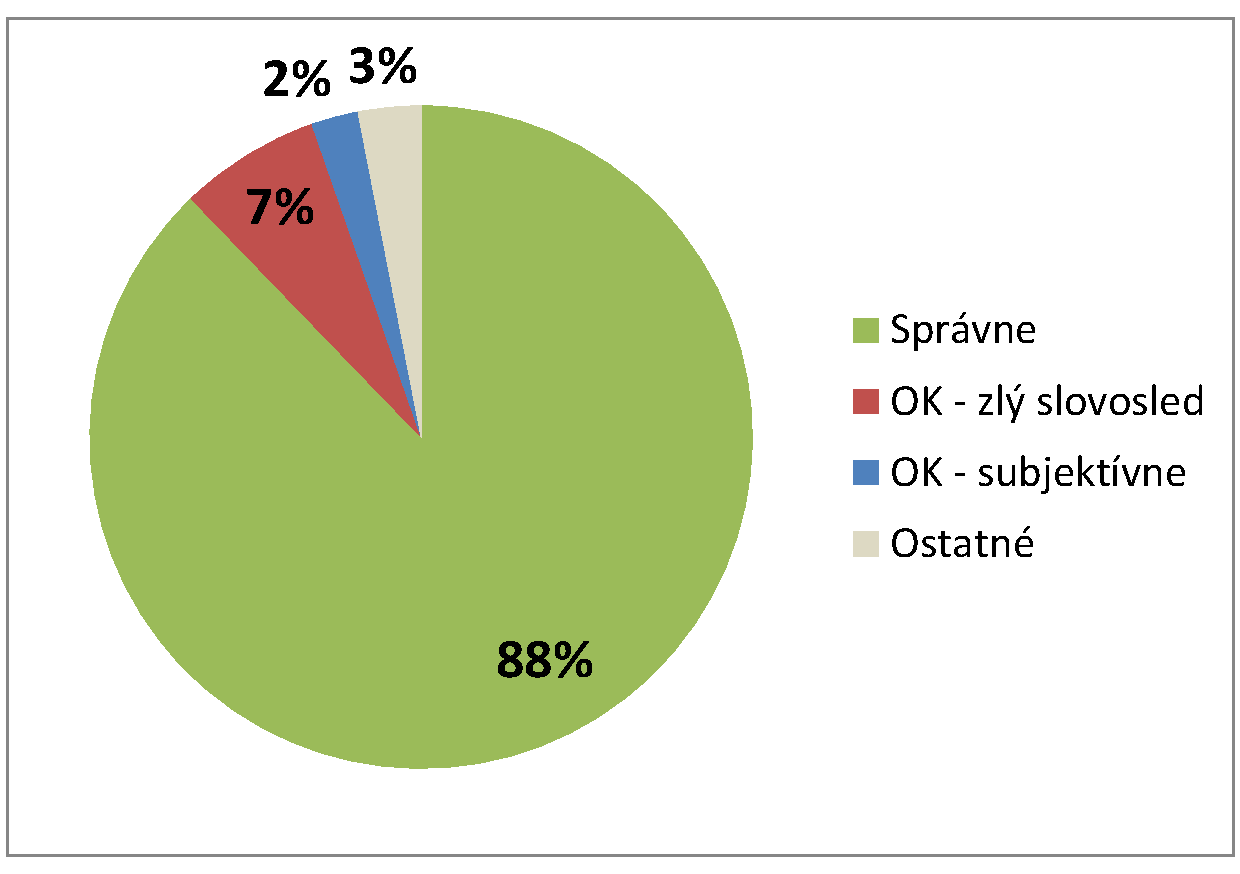
\includegraphics[scale=0.30]{exp_second_correct} }}%
	\caption{Detailné výsledky druhej časti experimentu}%
	\label{experiments:user_experiment:results:fig:exp_detailed_comparison_second}%
\end{figure}

\subsubsection{Vyhodnotenie experimentu}
Tvorba vyhovujúcich poznámok je subjektívna aktivita a preto hodnotenia účastníkov experimentu boli subjektívne a ovplyvnené ich predstavou o tvorbe poznámok. Avšak subjektívne hodnotenia boli objektívne roztriedené do kategórií a vyhodnotené. Z výsledkov je vidno $20\%$ zlepšenie z pohľadu počtu správne vytvorených poznámok pri použití databázy s väčším počtom pravidiel. V druhej časti je oproti prvej časti znížený počet zle spracovaných poznámok a poznámok, v ktorých chýbala podstatná informácia. Zväčšilo sa percentuálne zastúpenie kategórie \textit{chýba mala časť informácie}, čo naznačuje zlepšenie aj v prípade nesprávne vytvorených poznámok. V správne vytvorených poznámkach je v druhej časti väčšie percentuálne zastúpenie kategórie \textit{OK - zlý slovosled} oproti prvej časti. Taktiež nastali situácie kedy poznámka v prvej časti bola vytvorená správne a v druhej časti nesprávne. Spomenuté zhoršenia druhej časti oproti prvej súvisia s veľkou všeobecnosťou pravidla. Pravidlo sa aplikuje na vetu s rovnakou štruktúrou, ale rovnaká štruktúra môže mať viacero rôznych spracovaní.
% Z toho nám vyplynulo, že pravidlo príliš všeobecné a je potrebné aby bolo viac reštriktívne.

$80\%$ účastníkov experimentu podalo pozitívnu spätnú väzbu a vyjadrilo sa, že by takýto alebo podobný systém na tvorbu poznámok používali.

\subsection{Zhrnutie}
Na systéme boli vykonané tri experimenty. V prvom experiment sme náš systém porovnali so systémom Autosummarizer, ktorý sa špecializuje na sumarizáciu textu. Z tohto experimentu sa ukázalo, že náš systém posiela na výstup viacero viet a slov ako porovnávaný systém, čo môže mať za dôsledok veľké množstvo dát na výstupe pri rozsiahlejších článkoch. Na druhej strane náš systém spracoval všetky vety a eliminoval v nich irelevantné informácie. Druhý systém vynechal vety pri spracovávaní a tak isto neeliminoval irelevantné informácie z viet.

Druhým experimentom sme dokázali, že pravidlá sú dostatočne všeobecné, aby sa dali použiť na viacero viet s rovnakou štruktúrou. Tým sa nám podarilo ušetriť podstatnú časť prípadných pravidiel, ktoré by systém musel vytvoriť, ak by pre každú vetu potreboval samostatné pravidlo.

Pomocou používateľského experimentu sme overili systémovú závislosť od počtu pravidiel. Čím viac pravidiel má systém k dispozícií, tým kvalitnejšie spracováva vety, vytvára lepšie poznámky a stáva sa viac personalizovaný pre používateľa. Zaznamenali sme podstatné zlepšenie pri použití väčšieho množstva pravidiel v systéme. Z experimentu vyplynulo, že aj keď je poznámka spracovaná nesprávne, neznamená to, že je úplne nepoužiteľná pre používateľa. V podstatnej časti nesprávne vytvorených poznámok chýbala iba mala časť informácie z vety na to, aby bola úplne pochopiteľná a použiteľná pre používateľa. Počas experimentu sme odhalili situácie, kedy sa veta pri menšom počte pravidiel spracovala správne a pri väčšom počte nesprávne. Za dôsledok to má veľká všeobecnosť pravidla a je potrebné, aby bolo viac reštriktívne.